\documentclass{beamer}
\usetheme{Frankfurt}
\addtobeamertemplate{navigation symbols}{}{%
    \usebeamerfont{footline}%
    \usebeamercolor[fg]{footline}%
    \hspace{1em}%
    \insertframenumber/\inserttotalframenumber
}

\usepackage{mathtools}
\usepackage{graphicx}
\usepackage{braket}
\usepackage{amsthm}
\usepackage{lmodern}
\usepackage[utf8]{inputenc}
\usepackage[frenchb]{babel}
\usepackage[T1]{fontenc}
\usepackage{subcaption}
\usepackage{caption}
\usepackage{gensymb}
\usepackage{tikz}
\usepackage[qm]{qcircuit}
\usepackage{listings}
\usepackage{pgfplots}
\usepackage{xcolor}
\usepackage{amsmath}
\usepackage{color, colortbl,booktabs}
\usepackage[ruled,vlined]{algorithm2e}
\captionsetup[figure]{labelformat=empty}
\DeclareUnicodeCharacter{0301}{\'{e}}
\DeclareMathOperator{\tr}{tr}

\definecolor{mGreen}{rgb}{0,0.6,0}
\definecolor{mGray}{rgb}{0.5,0.5,0.5}
\definecolor{mPurple}{rgb}{0.58,0,0.82}
\definecolor{backgroundColour}{rgb}{0.95,0.95,0.92}
\definecolor{Gray}{gray}{0.9}
\lstdefinestyle{CStyle}{
    backgroundcolor=\color{backgroundColour},
    commentstyle=\color{mGreen},
    keywordstyle=\color{magenta},
    numberstyle=\tiny\color{mGray},
    stringstyle=\color{mPurple},
    basicstyle=\footnotesize,
    breakatwhitespace=false,
    breaklines=true,
    captionpos=b,
    keepspaces=true,
    numbers=left,
    numbersep=5pt,
    showspaces=false,
    showstringspaces=false,
    showtabs=false,
    tabsize=2,
    language=Python
}

\begin{document}

\makeatletter
\newcommand\titlegraphicii[1]{\def\inserttitlegraphicii{#1}}
\titlegraphicii{}
\setbeamertemplate{title page}
{
  \vbox{}
   {\usebeamercolor[fg]{titlegraphic}\inserttitlegraphic\hfill\inserttitlegraphicii\par}
  \begin{centering}
    \begin{beamercolorbox}[sep=8pt,center]{institute}
      \usebeamerfont{institute}\insertinstitute
    \end{beamercolorbox}
    \begin{beamercolorbox}[sep=8pt,center]{title}
      \usebeamerfont{title}\inserttitle\par%
      \ifx\insertsubtitle\@empty%
      \else%
        \vskip0.25em%
        {\usebeamerfont{subtitle}\usebeamercolor[fg]{subtitle}\insertsubtitle\par}%
      \fi%     
    \end{beamercolorbox}%
    \vskip1em\par
    \begin{beamercolorbox}[sep=8pt,center]{date}
      \usebeamerfont{date}\insertdate
    \end{beamercolorbox}
    \begin{beamercolorbox}[sep=8pt,center]{author}
      \usebeamerfont{author}\insertauthor
    \end{beamercolorbox}
  \end{centering}
}
\makeatother
\title{Conception de détecteurs quantiques optimaux via le calcul par intervalles}
\author{\tiny Pierre Engelstein, Nicolas Delanoue, François Chapeau-Blondeau}
\date{Journée du GdR CNRS ISIS - Traitement du signal et applications quantiques \\ 22 juin 2021}
\titlegraphic{\includegraphics[width=2cm]{images/LogoUnivAngers.png}}
% Ajouter logo LARIS a la place
\titlegraphicii{\includegraphics[width=1.8cm]{images/LogoLARIS.png}}

\begin{frame}[plain]
  \maketitle
  \tiny
\end{frame}

\begin{frame}
    \frametitle{Présentation du problème}
    % \tableofcontents
    \begin{block}{}
        On se place dans le problème de base du traitement du signal quantique consistant en la conception d'un détecteur quantique optimal maximisant la performance de détection d'un état parmi une famille d'états quantique, chaucn étant représenté par un opérateur densité $\rho_j$ et ayant une probabilité à priori $p_j$, étant mesuré via un opérateur de mesure $\Pi_k$.

        % \'Etant donné cette famille d'opérateurs densité $\{\rho_j, 1 \leq j \leq m\}$ et leur probabilités à priori, la famille d'opérateurs de mesure $\{\Pi_k, 1 \leq k \leq n \}$ permet de délivrer une certaine mesure $k$.
    \end{block}
\end{frame}

\section[Mesure quantique]{Mesure quantique optimale}

\begin{frame}
    \frametitle{Opérateur densité}
    \small

    \begin{block}{Définition}
        Un \textit{opérateur densité} pour un état quantique est une matrice Hermitiene $\rho$, telle que $\rho = \rho^{\dagger}$, de trace $\tr(\rho) = 1$ et semi-définie positive $\rho \succeq 0$.
    \end{block}

    \begin{columns}
        \begin{column}{0.5\textwidth}
            \begin{block}{Définition}
                Soit un système quantique dans un état \textbf{pur} $\ket{\phi_j}$.  L'opérateur densité correspondant à cet état est définit par:
        
                \begin{align}
                    \rho_j = \ket{\psi_j} \bra{\psi_j}.
                \end{align}
        
                L'opérateur densité est aussi capable de représenter des états \textbf{mixtes} qui ne sont pas représentables par les vecteurs d'états.
            \end{block}
        \end{column}
        \begin{column}{0.5\textwidth}
            \begin{block}{Exemple}
                Soit un état quantique $\ket{\psi_j} = \ket{+} = 
                \begin{bmatrix}
                    \frac{1}{\sqrt{2}} \\ \frac{1}{\sqrt{2}}
                \end{bmatrix}$
        
                L'opérateur densité correspondant est : 

                \begin{align}
                    \rho_j &= \ket{\psi_j}\bra{\psi_j} =\begin{bmatrix} \frac{1}{\sqrt{2}} \\ \frac{1}{\sqrt{2}} \end{bmatrix} \begin{bmatrix} \frac{1}{\sqrt{2}} & \frac{1}{\sqrt{2}} \end{bmatrix} \nonumber\\
                    &= \begin{bmatrix} 0.5 & 0.5 \\ 0.5 & 0.5 \end{bmatrix} \nonumber
                \end{align}
            \end{block}
        \end{column}
    \end{columns}
    % Ref. Vers les transparents de F. Chapeau-Blondeau
\end{frame}

\begin{frame}
    \frametitle{Opérateurs de mesure \footnote{Chapeau-Blondeau, F., "Quantum information, quantum computation : An introduction", Cours de formation doctorale (2018)}}

    \begin{block}{Définition}
        La \textit{mesure projective} est définie par un ensemble de $N$ projecteurs orthogonaux $\ket{n}\bra{n} = \Pi_n$, vérifiant $\displaystyle \sum_n\ket{n}\bra{n} = \displaystyle \Pi_n = I_N$ et $Pr\{\ket{n}\} = \tr(\rho \Pi_n)$.
    \end{block}

    \begin{block}{Définition: Mesure généralisée (POVM)}
        On généralise la notion de mesure projective à un ensemble non orthogonal d'opérateurs de mesure appelés POVM (\textit{positive operator-valued measurement}) $\{\Pi_n\}$ vérifiant $\displaystyle \sum_n \Pi_n = I_N$ et $Pr\{\Pi_n\} = \tr(\rho \Pi_n)$.
    \end{block}

    % Ref. Vers les transparents de F. Chapeau-Blondeau
\end{frame}

\begin{frame}
    \frametitle{Distribution des probabilités conjointes \footnote{Davies, E., "Information and quantum measurement", IEEE Transaction on Information Theory 24 (1978), 596-599}}
    \small
    \begin{block}{Définition}
        Soit un ensemble d'états quantiques $\{\rho_j\}$ avec leur probabilités $\{p_j\}$ tel que $\displaystyle \sum_j p_j = 1$.

        Considérons un ensemble correspondant de POVM $\{\Pi_k\}$ permettant de réaliser une mesure généralisée.

        La \textit{distribution des probabilités conjointes} entre la variable $X$ et la variable $Y$ est définie par :

        \begin{align}
            \Pr\{X = j, Y = k\} = P_{jk} = p_j \tr(\rho_j \Pi_k)
        \end{align}
    \end{block}

    \begin{block}{Interprétation}
        Un élément $P_{jk}$ correspond à la probabilité de mesurer $\Pi_k$ en ayant l'état quantique $\rho_j$.
    \end{block}
\end{frame}

\begin{frame}
    \frametitle{Critères d'optimisation}
    \begin{enumerate}
        \item Minimiser une combinaison linéaire des probabilités (cf. refs 6, 7, 9, 10, 15 davies)
        \item Maximiser la probabilité de détection correcte (linéaire), \footnote{\tiny Eldar, Y., "Designing Optimal Quantum Detectors Via Semidefinite Programming", IEEE Transaction on Information Theory 49 (2003), 1012-1017}
        \item Minimiser l'erreur quadratique de mesure, \footnote{\tiny Eldar, Y., "On Quantum Detection and the Square-Root Measurement", IEEE Transaction on Information Theory 47 (2001), 858-872}
        \item Maximiser information mutuelle \footnote{\tiny Davies, E., "Information and quantum measurement", IEEE Transaction on Information Theory 24 (1978), 596-599}.
    \end{enumerate}
\end{frame}

\begin{frame}
    \frametitle{Maximiser l'information mutuelle}

    \only<1>{
        \small
        \begin{block}{Définition}
            
            L'\textit{information mutuelle} est définie pour deux variables aléatoires $X$ et $Y$ par:

            \begin{align}
                I(X; Y) &= H(X) + H(Y) - H(X, Y) \\
                &= H(Y) - H(Y | X) \\
                &= H(X) - H(X | Y)
            \end{align}

            \begin{columns}
                \begin{column}{0.5\textwidth}
                    \tiny
                    \begin{enumerate}
                        \item $H(X)$ et $H(Y)$ entropies marginales de $X$ et $Y$; 
                        \item $H(X, Y)$ entropie conjointe de $X$ et $Y$;
                        \item $H(X|Y)$ entropie de $X$ sachant $Y$.
                    \end{enumerate}
                \end{column}
                \begin{column}{0.5\textwidth}
                    \tiny
                    \begin{align*}
                        X &= \{ \rho_j = \ket{\phi_j}\bra{\phi_j}, 1 \leq j \leq m\}, \nonumber\\
                        Y &= \{ \Pi_k  = \ket{\mu_k}\bra{\mu_k}, 1 \leq k \leq m\} \nonumber
                    \end{align*}
                    Avec $\{p_j\}$ distribution marginale de $X$.
                \end{column}
            \end{columns}

        \end{block}
        % \begin{block}{Définition}
        %     L'\textit{information mutuelle} est définie par rapport à la matrice des probabilités $P$:

        %     \begin{align}
        %         I(P) = \displaystyle \sum_{i} H(\displaystyle \sum_{j} P_{ij}) + \displaystyle \sum_{j} H(\displaystyle \sum_{i} P_{ij})  -\displaystyle \sum_{ij} H(P_{ij})
        %     \end{align}

        %     Avec $H(x) = -x \log(x)$ entropie de la variable $x$.
        % \end{block}
    }

    \only<2>{
        \begin{columns}
            \small
            \begin{column}{0.5\textwidth}
                \begin{block}{Problème}
                    On cherche à résoudre le problème de maximisation :
                    \begin{align}
                        \max\limits_{\{\Pi\}} I(\rho, \Pi)
                    \end{align}
        
                    tel que :
        
                    \begin{align}
                        \Pi_j \succeq 0, \quad 1 \leq j \leq m \label{eq:contrainte_sdp} \\
                        \displaystyle \sum_{j=1}^{m} \Pi_j = I \label{eq:contrainte_somme_id}
                    \end{align}
                \end{block}
            \end{column}
            \begin{column}{0.5\textwidth}
                \begin{figure}[H]
                    \centering
                    \includegraphics[scale=0.13]{images/MI_convex.png}
                    \caption{}
                    \label{fig:mi_convex}
                \end{figure}
            \end{column}
        \end{columns}


        \begin{itemize}
            \item Problème de maximisation de fonction convexe: difficile en pratique à résoudre.
            \item Utilisation du calcul par intervalle pour fournir une solution optimale garantie.
        \end{itemize}
    }
\end{frame}

\section[Calcul par intervalles]{Optimisation via le calcul par intervalle}
\begin{frame}
    \frametitle{Intervalles}
    \begin{block}{Notion d'intervalle}
        Un intervalle $\textbf{x} = [\underline{x}, \overline{x}]$ est défini comme l'ensemble des nombres réels $x$ t.q. $\underline{x} \leq x \leq \overline{x}$. 
    \end{block}

    \begin{block}{Notion de boites}
        Une boite $\textbf{X} = (\textbf{x1}, \textbf{x2}, ..., \textbf{xj})$ est le produit cartésien des intervalles $\textbf{x1} \times \textbf{x2} \times \dots \times \textbf{xj}$
    \end{block}

    \begin{figure}[H]
        \centering
        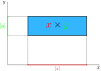
\includegraphics[scale=0.5]{images/box.png}
        \caption{}
        \label{fig:box}
    \end{figure}
\end{frame}

\begin{frame}
    \frametitle{Fonction d'inclusion}

    \begin{block}{Définition}
        Soit $f : \mathbb{R}^n \rightarrow \mathbb{R}^m$ une fonction, la fonction $[f] : \mathbb{R}^n \rightarrow \mathbb{R}^m$ est une \textit{fonction d'inclusion} pour $f$ si

        \begin{align}
            \forall[\underline{x}, \overline{x}] \in \mathbb{R}^n , f([\underline{x}, \overline{x}]) \subset [f]([\underline{x}, \overline{x}])
        \end{align}
    \end{block}

    \only<1>{
        \begin{figure}[H]
            \centering
            \includegraphics[scale=0.5]{images/function_eval_1.png}
            \caption{}
            \label{fig:fct1}
        \end{figure}
    }
    \only<2>{
        \begin{figure}[H]
            \centering
            \includegraphics[scale=0.5]{images/function_eval_2.png}
            \caption{}
            \label{fig:fct2}
        \end{figure}
    }
    \only<3>{
        \begin{figure}[H]
            \centering
            \includegraphics[scale=0.5]{images/function_eval_3.png}
            \caption{}
            \label{fig:fct3}
        \end{figure}
    }

    % Fonction d'inclusion forme centrée
\end{frame}


\begin{frame}
    \frametitle{Arithmétique des intervalles}
    On définit un ensemble d'opérateurs comme extension des opérateurs arithmétiques sur les nombres réels:

    \small
    \begin{itemize}
        \item $[x_1] + [x_2] = [\underline{x_1} + \underline{x_2}, \overline{x_1} + \overline{x_2}]$
        \item $[x_1] - [x_2] = [\underline{x_1} - \overline{x_2}, \overline{x_1} - \underline{x_2}]$
        \item $[x_1] \times [x_2] = [\text{min}(\underline{x_1}\underline{x_2}, \underline{x_1}\overline{x_2}, \overline{x_1}\underline{x_2}, \overline{x_1}\overline{x_2}), \text{max}(\underline{x_1}\underline{x_2}, \underline{x_1}\overline{x_2}, \overline{x_1}\underline{x_2}, \overline{x_1}\overline{x_2})]$
        \item $\log([x]) = [\log(\underline{x_1}), \log(\overline{x_2})]$
        \item \dots
    \end{itemize}

    \begin{block}{Exemple}
        \begin{align}
            [z] &= ([2, 3] - [-4, 5])^2 + [-3, 2] \nonumber \\
                &= [-3,7]^2 + [-3, 2] \nonumber \\
                &= [0, 49] + [-3, 2] \nonumber \\
                &= [-3, 51] \nonumber
        \end{align}
    \end{block}
\end{frame}

\begin{frame}
    \frametitle{Petite histoire du calcul par intervalle \footnote{\tiny Delanoue, N., "Méthodes numériques garanties pour la classification de fonctions et le contrôle optimal", Soutenance HDR, 2018}}
    \begin{block}{}
        \small
        \begin{enumerate}
            \item Arithmétique des intervalles, R. E. Moore, 1966,
            \item Optimisation globale, R. Baker Kearfott, 90’s,
            \item Résolution de systèmes d’équations, A. Neumaier, 90’s,
            \item Résolution d’équations différentielles ordinaires, R. Lohner 1988,
            \item La preuve de l’existence de l’attracteur étrange pour le système de Lorentz, W. Tucker, 1998,
            \item Analyse par intervalles appliquée à la robotique, L. Jaulin, 2001,
            \item La preuve de la conjecture de Kepler, T. Hales, 2003,
            \item Estimation de paramètres pour les systèmes décrits par les équationsdifférentielles ordinaires, N. Ramdani, 2004,
            \item EDP, topologie algébrique, \dots
        \end{enumerate}
    \end{block}
\end{frame}

\begin{frame}
    \frametitle{Premier algorithme d'optimisation}
    \begin{block}{Théorème}
        Soit un $a$ une solution admissible du problème $\max\limits_{x} f(x)$ tel que $g(x) \leq 0$ et $x^*$ la solution optimale, on a:
        \begin{align}
            sup([f]([x])) \leq f(a) \Rightarrow x^* \notin [x]
        \end{align}
    \end{block}

    \only<1>{
        \begin{figure}[H]
            \centering
            \includegraphics[scale=0.5]{images/function_optim_1.png}
            \caption{$y = f(x)$}
            \label{fig:optim1}
        \end{figure}
    }

    \only<2>{
        \begin{figure}[H]
            \centering
            \includegraphics[scale=0.5]{images/function_optim_2.png}
            \caption{$y = f(x)$}
            \label{fig:optim2}
        \end{figure}
    }

    \only<3>{
        \begin{figure}[H]
            \centering
            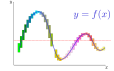
\includegraphics[scale=0.5]{images/function_optim_3.png}
            \caption{$y = f(x)$}
            \label{fig:optim3}
        \end{figure}
    }

    \only<4>{
        \begin{figure}[H]
            \centering
            \includegraphics[scale=0.5]{images/function_optim_4.png}
            \caption{$y = f(x)$}
            \label{fig:optim4}
        \end{figure}
    }

    \only<5>{
        \begin{figure}[H]
            \centering
            \includegraphics[scale=0.5]{images/function_optim_5.png}
            \caption{$y = f(x)$}
            \label{fig:optim5}
        \end{figure}
    }

    \only<6>{
        \begin{figure}[H]
            \centering
            \includegraphics[scale=0.5]{images/function_optim_6.png}
            \caption{$y = f(x)$}
            \label{fig:optim6}
        \end{figure}
    }

    \only<7>{
        \begin{figure}[H]
            \centering
            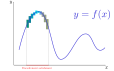
\includegraphics[scale=0.5]{images/function_optim_7.png}
            \caption{$y = f(x)$}
            \label{fig:optim7}
        \end{figure}
    }

\end{frame}

\begin{frame}
    \frametitle{Algorithme avancé}

    Quatres étapes pour l'algorithme, itérativement:
    \begin{itemize}
        \item Bisection d'une boite selon un axe donné (plus grand axe par exemple);
        \item \'Evaluation des contraintes sur les boites résultantes: permet d'éliminer les boites hors-contraintes;
        \item Borner la fonction avec le calcul par intervalle;
        \item Choix d'un candidat $a$ pour l'élimination par borne supérieure (point milieu, recherche d'un maximum dans l'intervalle avec un algorithme classique, \dots)
    \end{itemize}
\end{frame}

\section[Application à la mesure optimale]{Application à la mesure optimale}
\begin{frame}
    \frametitle{Exemple concret}
    \tiny
    \begin{block}{}
        Considérons deux états purs $\ket{\psi_1} = \begin{bmatrix}\frac{1}{3} \\ \frac{2 \sqrt(2)}{3}\end{bmatrix}$ et $\ket{\psi_2} = \ket{+}$, avec $p_1 = 0.1$ et $p_2 = 0.9$.

        Les opérateurs densité correspondant sont:

        \begin{align}
            \rho_1 = \begin{bmatrix}
                \frac{1}{9} & \frac{2 \sqrt{2}}{9} \\ \frac{2 \sqrt{2}}{9} & \frac{8}{9}
            \end{bmatrix}, 
            \quad \rho_2 = \begin{bmatrix}
                0.5 & 0.5 \\ 0.5 & 0.5
            \end{bmatrix} \nonumber
        \end{align}

        \medbreak
        
        Et on a deux opérateurs de mesure inconnus soit 8 variables inconnues:

        \begin{align}
            \Pi_1 = \begin{bmatrix}
                a_1 & b_1 + ic_1 \\ b_1 - ic_1 & d_1
            \end{bmatrix}, \quad \Pi_2 = \begin{bmatrix}
                a_2 & b_2 + ic_2 \\ b_2 - ic_2 & d_2
            \end{bmatrix} \nonumber
        \end{align}

        Le critère de Shannon maximum est $-0.1\log_2(0.1) - 0.9\log_2(0.9) = 0.469.$ 

    \end{block}
\end{frame}

\begin{frame}
    \frametitle{Exemple concret}
    \tiny
    \begin{block}{}
        On veut résoudre le problème 
        \begin{align}
            &\max\limits_{\Pi_1, \Pi_2} I(\rho_1, \rho_2, \Pi_1, \Pi_2) \\
            % &= -(\tr(\rho_1 . \Pi_1) + \tr(\rho_1 . \Pi_2))\log(\tr(\rho_1 . \Pi_1) + \tr(\rho_1 . \Pi_2)) \\
            % &- (\tr(\rho_2 . \Pi_1) + \tr(\rho_2 . \Pi_2))\log(\tr(\rho_2 . \Pi_1) + \tr(\rho_2 . \Pi_2)) \\
            % &-(\tr(\rho_1 . \Pi_1) + \tr(\rho_2 . \Pi_1))\log(\tr(\rho_1 . \Pi_1) + \tr(\rho_2 . \Pi_1)) \\
            % &- (\tr(\rho_1 . \Pi_2) + \tr(\rho_2 . \Pi_2))\log(\tr(\rho_1 . \Pi_2) + \tr(\rho_2 . \Pi_2))
% 
\Leftrightarrow \max\limits_{\Pi_1, \Pi_2} \big(&-(\alpha_{11} + \alpha_{12})\log(\alpha_{11} + \alpha_{12}) - (\alpha_{21} + \alpha_{22})\log(\alpha_{21} + \alpha_{22}) \nonumber \\
             &- (\alpha_{11} + \alpha_{21})\log(\alpha_{11} + \alpha_{21}) - (\alpha_{12} + \alpha_{22})\log(\alpha_{12} + \alpha_{22}) \nonumber \\
             &+ (\alpha_{11})\log(\alpha_{11}) + (\alpha_{12})\log(\alpha_{12}) + (\alpha_{21})\log(\alpha_{21}) + (\alpha_{22})\log(\alpha_{22}) \big),\nonumber\\
             &\alpha_{jk} = \tr(\rho_j . \Pi_k) \nonumber
        \end{align}

        tel que :

        \begin{align}
            \Pi_1 \succeq 0, \Pi_2 \succeq 0\\
            \Pi_1 + \Pi_2 = I 
        \end{align}

    \end{block}
\end{frame}

\begin{frame}
    \frametitle{Exemple concret}
    \small
    \begin{block}{}


        On sait que $\Pi_1 + \Pi_2 = I_2$, on réduit à 4 variables inconnues:

        \begin{align}
            \Pi_2 = \begin{bmatrix}
                (1-a_1) & (-b_1) + i(-c_1) \\ (-b_1) - i(-c_1) & (1-d_1)
            \end{bmatrix} \nonumber
        \end{align}

        Comme les $\rho_i$ ne comportent pas de termes complexes, on peut retirer le terme $c$ des $\Pi_j$, on réduit à 3 variables $\{a, b, d\}$ notre problème.

        On pose les contraintes de Silvester pour la contrainte de semi-définition positive des opérateurs de mesure:

        \begin{align}
            a \geq 0 \nonumber \\
            d \geq 0 \nonumber \\
            a \times d - b^2 \geq 0 \nonumber \\
            (1-a) \times (1-d) - (-b)^2 \geq 0 \nonumber
        \end{align}
    \end{block}
\end{frame}

% Résultats (ibex / le notre)


\begin{frame}
    \frametitle{Résultats}

    \begin{block}{Ibex}
        Ibex nous donne un criètre de Shannon de $0.156$ avec une précision relative de $0.001$, et
        
        $\Pi_1 = \begin{bmatrix} 0.454 & -0.498 \\ -0.498 & 0.546 \end{bmatrix}$, \quad $\Pi_2 = \begin{bmatrix}0.546 & 0.498 \\ 0.498 & 0.454 \end{bmatrix}$.

        Le temps de calcul est de 124 secondes.
    \end{block}

    \begin{block}{Notre solveur}
        Notre solveur nous donne un criètre de Shannon de $0.156$ avec une précision relative de $4\times 10^{-9}$, et
        
        $\Pi_1 = \begin{bmatrix} 0.456 & -0.498 \\ -0.498 & 0.544 \end{bmatrix}$, \quad $\Pi_2 = \begin{bmatrix}0.544 & 0.498 \\ 0.498 & 0.456 \end{bmatrix}$.

        Le temps de calcul est de 13 secondes.
    \end{block}

\end{frame}


\section[Perspectives]{Perspectives}
\begin{frame}
    \frametitle{Perspectives}
    \begin{enumerate}
        \item \'Etendre le problème à des états d'entrée bruités: on considère alors les $\{\rho\}$ comme étant inconnus;
        \item Difficulté d'étendre le problème à des dimensions supérieures: complexité exponentielle avec la dimension.
        \item L'algorithme étant parallélisable, on peut néanmoins réduire considérablement le temps de calcul, en fonction du nombre de processeurs.
    \end{enumerate}
\end{frame}

% Perspectives: Etendre le problème à états d'entrée inconnus - bruités

% Algo parallélisable : réduction considérable du temps de calcul dépendant du nombre de processeurs

% On arrive pas à converger dans certains cas => explosion combinatoire

\end{document}